\input{settings}
\setlength{\emergencystretch}{2em}
\titleformat{\section}
  {\small\bfseries\raggedright}
  {}{0em}
  {}
  [{\color{WHU_Blue}\titlerule}]
\titlespacing*{\section}{0cm}{0.85em}{0.60em}
\titlespacing*{\subsection}{0cm}{0.50em}{0.30em}
\setlist[itemize]{topsep=0.20em, itemsep=0.20em, parsep=0em, partopsep=0em, leftmargin=1.25em}
\setlist[enumerate]{topsep=0.20em, itemsep=0.20em, parsep=0em, partopsep=0em, leftmargin=1.35em}
\renewcommand{\arraystretch}{0.98}
\renewcommand{\CJKglue}{\hskip 0.018em}

% 个人信息
%  cd C:\Users\31087\Documents\Obsidian_Vault\Resume\template
%  xelatex main_ant.tex
\newcommand{\school}{江南大学 · 控制科学与工程}

\newcommand{\resumeDecor}{
    \begin{tikzpicture}[remember picture, overlay]
        \node[anchor=north, inner sep=0pt](header) at (current page.north){
            
\includegraphics[width=\paperwidth]{images/header.png}
        };
        \node[anchor=west](school_logo) at (header.west){
            \hspace{0.5cm}
            
\includegraphics[width=0.15\textwidth]{images/whu_logo_1.png}
        };
        \node[anchor=east](school_name) at(header.east){
            \textcolor{white}{\textbf{\school}}
            \hspace{0.5cm}
        };
    \end{tikzpicture}

    \begin{tikzpicture}[remember picture, overlay]
        \node[opacity=0.05] at(current page.center){
            
\includegraphics[width=0.68\paperwidth, keepaspectratio]{images/whu_logo_big.png}
        };
    \end{tikzpicture}
}

\newcommand{\sectionIcon}[2]{\makebox[\widthof{#1}][c]{\color{WHU_Blue}{#1}}\quad #2}

%%%%%%%%%%%%%%%%%%%%
% 简历正文
%%%%%%%%%%%%%%%%%%%%
\begin{document}
\resumeDecor
\vspace*{-3.15em}
\scriptsize
\linespread{1.10}\selectfont

\begin{minipage}{0.80\textwidth}
    \section[个人信息]{\sectionIcon{\faAddressCard}{个人信息}}
    \footnotesize
    \begin{tabularx}{\linewidth}{p{\widthof{求职意向:}}Xp{\widthof{最高学历:}}X}
        姓\ \ \ \ \ \ \ \ 名: & 梁邦一 &
        性\ \ \ \ \ \ \ \ 别: & 男 \\
        邮\ \ \ \ \ \ \ \ 箱: & yuejinai55@gmail.com &
        电\ \ \ \ \ \ \ \ 话: & +86 15515602693 \\
        英语等级: & CET-6 &
        求职意向: & 具身智能算法工程师（2027届校招） \\
        & &
    \end{tabularx}
\end{minipage}
\hfill
\begin{minipage}{0.11\textwidth}
    \vspace{2.0em}
    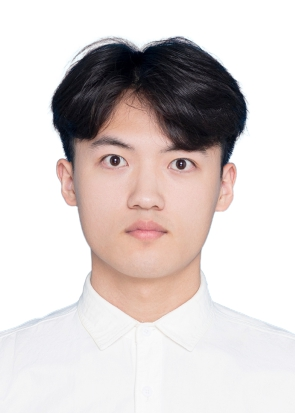
\includegraphics[width=\linewidth]{images/avatar.png}
\end{minipage}
\vspace{-0.60em}

% \section[个人总结]{\sectionIcon{\faBook}{个人总结}}
% 控制科学与工程硕士在读，本科自动化背景，围绕机器人感知、人机交互、多模态传感、机械臂/末端灵巧手遥操作和 VLA 真机/仿真实践开展研究，具备从感知输入、模型输出到动作验证的完整链路理解。\\
% 基于 PyTorch 参与 Transformer / 轻量级 Conformer / YOLO11s-seg 等模型实验，做过视觉、肌电、压力等多通道数据同步采集、清洗标注、训练配置管理和 bad case 分析，理解数据质量、模型结构和泛化稳定性之间的关系。\\
% 在 NVIDIA Jetson AGX Orin 端侧完成感知模型部署与 TensorRT 推理加速（推理延迟降低 20\%），并参与 CARIZON 智驾感知数据挖掘实习，做过 Qwen3-VL / vLLM / 结构化打标 / 评估脚本和两阶段目标挖掘闭环，具备将 VLM 刷库、标签体系和自动化评测迁移到机器人多模态数据 pipeline 的基础。\\
% 持续关注 Imitation Learning、RL、Diffusion Policy、OpenVLA 等具身智能方向，具备英文论文研读、技术路线梳理和跨角色协作推进能力，能够快速进入机器人实验和工程联调节奏。

\section[教育背景]{\sectionIcon{\faGraduationCap}{教育背景}}
\begin{itemize}
    \item {\textbf{控制科学与工程硕士，江南大学}}（\hl{中国科学院沈阳自动化研究所 · 机器人与智能系统全国重点实验室联合培养}） \hfill {2024.06--2027.06}
    \item {\textbf{自动化学士，郑州轻工业大学}} \hfill {2020.09--2024.06}
\end{itemize}

\section[荣誉与组织经历]{\sectionIcon{\faStar}{荣誉与组织经历}}
\begin{itemize}
    \item {\textbf{荣誉奖项}}：中国机器人大赛暨 RoboCup 机器人世界杯中国赛（无人车组）\hl{国家三等奖}；校一等奖学金（2025.10、2026）；优秀毕业生（2024.06）；优秀班干部（2022.10）。
    \item {\textbf{组织经历}}：本科班长（2020.10-2024.06）；硕士党支部书记（2024.10-2026.05），具备跨角色沟通、任务分解和协作推进经验。
\end{itemize}

\section[专业技能]{\sectionIcon{\faWrench}{专业技能}}
\begin{itemize}
    \item \textbf{算法与模型}：PyTorch、Transformer、轻量级 Conformer、YOLO11s-seg、目标检测、实例分割、分类、连续值回归、时序信号建模、多模态特征融合。
    \item \textbf{端侧部署}：TensorRT、ONNX、NVIDIA Jetson AGX Orin、模型量化与算子优化。
    \item \textbf{机器人与仿真}：ROS2（Python / C++）、Topic 通信、灵巧手遥操作、机器人端联调、MuJoCo、Gazebo、VLA 真机与仿真、OpenVLA2。
    \item \textbf{数据工程}：多通道传感数据采集、清洗与标注、训练/验证/测试集划分、vLLM 批量推理、JSON 标签解析、Precision / Recall / F1 / 混淆矩阵评估。
    \item \textbf{工程环境}：Python、C++、Linux / Ubuntu、Git、bash。
\end{itemize}

\section[实习经历]{\sectionIcon{\faBriefcase}{实习经历}}
{\small\textbf{CARIZON（大众×地平线合资智驾）}}\quad 感知数据部门算法实习生 \hfill {2026.06--至今} \\
{\scriptsize\color{WHU_Blue} 感知数据闭环 / VLM 后训练 / 长尾场景挖掘}
\begin{itemize}
    \item 面向驾驶场景视觉目标，采用 Grounding DINO 开放词汇检测 + 专用 VLM 细粒度属性识别的组合方案，结合视觉 Embedding 检索构建相似样本召回链路，\hl{服务长尾样本挖掘、Corner Case 筛选与标签库建设}。
    \item 融合车载多路传感器与回灌数据设计规则化挖掘算子，红绿灯自车转向 Tagger 在 3W 条路口数据中筛选 3K 条 CLIP，\hl{标签验收准确率达 90\%、挖掘召回提升 10\%}，支撑感知模型训练与迭代。
    \item 负责感知细粒度识别 VLM 后训练优化：围绕闸机杆 / 限高杆五分类任务，完成数据清洗、标注校验与 Prompt 迭代，基于 Qwen3-VL-8B / Qwen3.5-9B + LLaMA-Factory 完成 13 轮 SFT 实验迭代与 H20 8GPU 集群全参数 SFT，\hl{测试集准确率 0.8984 创历史新高}；在 GT 生产平台落地 CoT 标注工具链，形成“人工标注 $\rightarrow$ SFT 训练数据”闭环。
\end{itemize}

\vspace{0.30em}
{\small\textbf{优奇智能科技有限公司（优必选子公司）}}\quad 人形机器人感知算法实习生 \hfill {2026.02--2026.05} \\
{\scriptsize\color{WHU_Blue} 端侧部署与推理加速 / 目标检测与实例分割 / 数据质检与 bad case 归因}
\begin{itemize}
    \item 负责 R11 接待机器人感知模型在 NVIDIA Jetson AGX Orin 端侧计算平台的部署，围绕 TensorRT 完成 PyTorch $\rightarrow$ ONNX $\rightarrow$ TensorRT 模型转换、量化与算子性能优化，\hl{推理延迟降低 20\%}，在真机跑通检测/分割实时推理链路，形成\hl{“训练—部署—实机验证”端到端工程闭环}。
    \item 参与 R11 接待机器人 YOLO11s-seg 模型训练复现，基于 Python / PyTorch / Ultralytics YOLO 在 Ubuntu 环境完成实验环境搭建、数据配置与训练参数调整，\hl{推动检测/分割训练链路跑通}。
    \item 参与多场景视觉数据清洗、标注质检与训练/验证/测试集划分；面向真实机器人场景归纳误检、漏检与分割边界不稳定等 bad case，形成问题清单与数据补充建议，\hl{将模型效果问题转化为可执行的数据侧优化需求}。
\end{itemize}

\section[科研与项目经历]{\sectionIcon{\faFlask}{科研与项目经历}}
{\small\textbf{面向具身智能灵巧操作的肌电-力融合感知与灵巧手抓取控制系统（灵心巧手） · 负责人}} \hfill {2025.02--2026.02} \\
{\scriptsize\color{WHU_Blue} 承载平台：机器人与智能系统全国重点实验室（中国科学院沈阳自动化研究所），江南大学联合培养}
\begin{itemize}
    \item 面向自然抓取示教中触觉手套改变手部接触体验的问题，提出“sEMG 意图力前馈 + 机器人端触觉闭环”的灵巧手抓取方案；搭建 Delsys Trigno sEMG + Sensel 压力 + 视觉多模态同步采集链路，完成抓取任务配置、会话标注、CSV 落盘与实时可视化，\hl{形成可复现实验数据入口}。
    \item 基于 PyTorch 推进 Transformer / 轻量 Conformer 肌电—力映射实验，支持\hl{力等级分类与连续力值回归双任务}；设计视觉—MuJoCo—sEMG—触觉分层控制链路，通过 ROS2 对接 Linker Hand G20，完成 Web/VR 演示与模块化接口沉淀，构成 \hl{Sim-to-Real 端到端方案雏形}。
    \item 围绕 ROS2 topic 设计模块化实验接口，梳理抓取状态、base pose、目标力、触觉反馈与关节位置命令的数据流，使视觉、仿真策略、肌电力估计与触觉控制模块能够独立替换、调试和验证。
    \item 在实验室承担课题实验链路组织与训练环境保障：负责传感器准备、通道配置、训练配置管理与结果检查，独立完成 \hl{Linux 服务器环境搭建与维护}；系统梳理手势识别、人机交互与机器人感知方向英文文献，\hl{支撑 IEEE Sensors Journal 综述写作}与技术路线判断。
\end{itemize}

\section[论文与研究成果]{\sectionIcon{\faBook}{论文与研究成果}}
\begin{itemize}
    \item \hl{已录用 · 第一作者}（JCR 一区 / 中科院二区） Liang B., Li N., Li G., et al. \textit{Sensing Technologies for Hand Gesture Recognition in Human-Robot Interaction: A Review}. IEEE Sensors Journal, 2025, 26(2): 1501-1519. \textbf{综述}：梳理数据手套、视觉与肌电等手势感知路线，对比精度、侵入性与成本取舍。
    \item \hl{In Revision（在修）}（JCR 一区 / 中科院二区 Top） \textit{sEMG Conformer: Synergizing Local-Global Spatiotemporal Features for Continuous Force Estimation}. Biomedical Signal Processing and Control. \textbf{算法核心}：卷积局部感受野 + 自注意力全局建模，解码肌电—指尖力映射，单模型支持力等级分类与连续力值回归。
    \item \hl{Under Review（在投）}（JCR 一区 / 中科院二区） \textit{Dexterous Hand Grasping Control Based on Multimodal Sensory Fusion and Simulation Reinforcement Learning}. \textbf{系统闭环}：MuJoCo 仿真强化生成抓取姿态，融合视觉、肌电与触觉构建分层控制链路，G20 上完成闭环部署验证。
\end{itemize}


\end{document}
